%

\section{Partial Epistemic Model for Epistemic Logic}
\label{sec:partialEpiModel}

%

%

%
%
%

Throughout this paper, we assume a distributed system consisting of $n$ ($n>1$) agents, 
which are distinguished by the identifiers taken from the set $\Ag = \{0, \ldots, n-1 \}$.
We say `agent~$a$' to refer to the agent with id $a \in \Ag$. 
%
%


%
%
%

\subsection{Topological model of distributed computing}
\label{subsec:topModelDistComp}

%
%
%

In the topological method \cite{Book:2013:HerlihyKozlovRajsbaum}, 
distributed systems are modeled by simplicial complexes. 
A global state of a distributed system is modeled 
by a \keywd{simplex}, i.e., a nonempty set of vertexes, where each vertex
represents the local state of a particular agent.
The nonderteministic set of global states of a distributed system is 
modeled by a \keywd{simplicial complex}, a set of simplexes that is closed 
under set inclusion. 
The topological model uses the so called \emph{chromatic}
simplicial complex, whose vertexes are properly `colored' with agent ids. 

\begin{definition}[chromatic simplicial complex]
    A \keywd{chromatic simplicial complex} $\cplC$ is a triple $\Tuple{V, S, \coloring}$ consisting
    of a set $V$ of vertexes, a set $S$ of \keywd{simplexes}, 
    and a \keywd{coloring map} $\coloring: V \zto \Ag$ that satisfy:
    \begin{itemize}
        \item $S$ is the set of simplexes, i.e., a set of nonempty subsets of $V$ 
        such that $X\in S$ and $\emptyset\subsetneq Y\subseteq X$ implies $Y \in S$;
        %
        \item For every $X \in S$ and $u,v\in X$, $\coloring(u)=\coloring(v)$ implies $u=v$.
    \end{itemize}

\end{definition}

For brevity, we often write complexes (resp., simplexes) to mean chromatic simplicial complexes (resp., chromatic simplexes).

%

A simplex $X$ is of dimension $d$, if $\Abs{X} =d+1$.
The dimension of a complex $\cplC$ is the maximum dimension of the simplexes contained in $\cplC$. 
A simplex $X$ is called a \keywd{facet} of $\cplC$, if 
$X$ is a maximal simplex, i.e., $\cplC$ contains no facet that is properly larger than $X$. 
We write $\Facet(\cplC)$ for the set of facets of $\cplC$.
%
A complex is called \keywd{pure} (of dimension $n-1$) if all facets are of the same dimension~$n-1$;
otherwise, the complex is called \keywd{impure}.
An impure complex contains a facet of dimension less than $n-1$. 
Such a facet represents a global state of the distributed system 
where some agents are `dead' due to crash. 

%
%
%
%
%
%

%
%
%

Given complexes $\Complex = \Tuple{V, S, \coloring}$ and $\Complex' = \Tuple{V', S', \coloring'}$,
a \keywd{simplicial map} $\delta:\cplC\to\cplC'$ is a color-preserving
map from $V$ to $V'$ such that:
\begin{itemize}
    \item $f(X) \in S'$ for every $X\in S$;
    \item $\coloring'(f(v)) = \coloring(v)$ for every $v \in V$.
\end{itemize}


%
%
%
%
%
%
%
%

%
%
%
%

%
%
%
%
%
%


%
%
%





%
%
%
%


\subsection{Partial epistemic model semantics for epistemic logic}
\label{subsec:partialEpistemicModel}

We are concerned with the analysis of distributed computability 
with epistemic logic \cite{Book:2004:JosephMoses}, a propositional logic augmented with a knowledge modality. 

\begin{definition}[The syntax of epistemic logic] \label{def:SyntaxEpistemicLogic}
    We assume the set $\At$ is a disjoint union of 
    atomic propositions indexed by agents, i.e., $\At =\bigcup_{a\in\Ag} \At_a$. 
    %
    %
    %
    %
    For $A \subseteq \Ag$, we write $\At_A$ for the set
    $\bigcup_{a \in A} \At_a$ of atomic propositions concerning the subset $A$ of agents.

    The set $\ModLangK$ of epistemic logic formulas are defined by the following BNF grammar:
    \[
        \varphi ::=
        p
        \mid \neg \varphi
        \mid \varphi \wedge \varphi \mid \varphi \vee \varphi
        \mid \ModK{a}{\varphi}
        \qquad (p \in \At,\: a \in \Ag).
    \]

    As usual, the implication $\varphi \zthen \varphi'$ is logically equivalent to $\neg \varphi \vee \varphi'$
    and $\Pfalse$ to $p\wedge \neg p$, for some $p\in\At$.  
    For a finite set of formulas $G = \{\varphi_1, \cdots, \varphi_k\}$, we write 
    $\bigwedge G$ for $\bigwedge_{i=1}^k \varphi_i$ 
    and $\bigvee G$ for $\bigvee_{i=1}^k \varphi_i$. 

%
%

    For $a\in \Ag$ and $B\subseteq \Ag$, 
    we write $\Paliveop{a}$ to abbreviate the formula $\neg \ModK{a} \Pfalse$ 
    and also $\Paliveop{B}$ to abbreviate $\bigwedge_{a \in B} \Paliveop{a}$. 
    The formula $\Paliveop{a}$ (resp., $\Paliveop{B}$) is intended to 
    describe that agent $a$ (resp., all agents in $B$) are alive. 

    In the subsequent discussion, we are concerned with a particular subclass $\ModLangKPlus$ 
    of formulas, called \keywd{guarded positive epistemic formulas}, given by:
    \[
        \varphi ::=
        \Paliveop{B} \zthen \psi
        \mid \varphi \wedge \varphi
        \mid \varphi \vee \varphi
        \mid \ModK{a}{\varphi}
        \qquad (a \in \Ag,~ B \subseteq \Ag),
    \]
    where $\psi$ ranges over pure propositional formulas whose atomic formulas 
    are restricted to those concerning agents in $B$, namely, 
    \[
        \psi ::=
        p
        \mid \neg \psi
        \mid \psi \wedge \psi
        \mid \psi \vee \psi
        \qquad (p \in \At_B).
    \]
\end{definition}


%
%
%
%
%
%
%
%
%
%

%
%
%
%
%
%
%
%
%
%
%
%
%
%
%
%
%
%
%
%
%
%
%
%
%
%
%
%
%



%


Following \cite{STACS22:GoubaultLedentRajsbaum}, 
below we define the semantics of epistemic logic in a partial epistemic model.

\begin{definition}[partial epistemic model] \label{def:PEframe}\label{def:PEmodel}
    A \keywd{partial epistemic frame} $\Tuple{W, \sim}$ is a pair consisting of:
    \begin{itemize}
        \item A nonempty finite set $W$ of possible worlds;
        \item An \keywd{indistinguishability relation} $\sim$, 
        which is a family of binary relations $\{ {\sim_a} \}_{a\in\Ag}$ over $W$  
        where each $\sim_a$ is a \keywd{partial equivalence relation} (PER), i.e., 
        $\sim_a$ is a symmetric and transitive, but not necessarily reflexive relation.
    \end{itemize}

    A \keywd{partial epistemic model} $\Mepistemic=\Tuple{W, \sim, L}$ 
    is a triple 
    that augments a partial epistemic frame $\Tuple{W, \sim}$ with a function $L: W \to \PowerSet{\At}$.
    The function $L$ assigns a set $L(w)$ of true atomic propositions to each world $w \in W$.
\end{definition}

When $w \sim_a w'$ holds in a partial epistemic model,     
it means that agent $a$ is alive in
both of the possible worlds $w$ and $w'$ and it cannot distinguish between these worlds.
Particularly, $w \not\sim_a w$ implies that
an agent~$a$ is dead in a possible world $w$.
We write $\Alives{w}$ for the set of agents that is alive in $w$, 
i.e., $\Alives{w} = \{ a \in \Ag \mid w \sim_a w \}$. 
%
For $A\subseteq\Ag$, we also write $w \sim_A w'$ to mean
$w \sim_a w'$ for every $a\in A$. 

%
%
Partial epistemic models generalize the usual epistemic models: 
Indistinguishability relations are given by equivalence relations instead of PERs,
which means that every agent is alive in epistemic models.


%
%
%
%


%
%

%
%
%
%
%
%

%
%
%


\begin{definition}
    Let $\Mepistemic = \Tuple{W, \sim, L }$ be
    a partial epistemic model.
    Given $w \in \Mepistemic$
    and $\varphi \in \ModLangK$,
    the satisfaction relation $\Mepistemic, w \models \varphi$,  
    which reads $\varphi$ is true in the possible world $w$ of $\Mepistemic$, 
    is defined by induction on the structure of $\varphi$ as follows.
    \begin{align*}
        \Mepistemic, w \models p
         &\quad \text{ iff } \quad p \in L(W)       \\
        \Mepistemic, w \models \neg \varphi
         &\quad \text{ iff } \quad \Mepistemic, w \not\models \varphi                                      \\
         \Mepistemic, w \models \varphi \wedge \varphi'
         &\quad \text{ iff } \quad \Mepistemic, w \models \varphi \text{ and } \Mepistemic, w \models \varphi' \\
         \Mepistemic, w \models \varphi \vee \varphi'
         &\quad \text{ iff } \quad \Mepistemic, w \models \varphi \text{ or } \Mepistemic, w \models \varphi' \\
        \Mepistemic, w \models \ModK{a}{\varphi}
         &\quad \text{ iff } \quad \Mepistemic, w' \models \varphi
        \text{ for every $w' \in W$ satisfying $w \sim_a w'$}.
    \end{align*}

    We write $\Mepistemic \models \varphi$ to mean $\varphi$ is \keywd{valid} in $\Mepistemic$, 
    i.e., $\Mepistemic, w \models \varphi$ for every $w\in W$. 
\end{definition}

%

%
%
%
%

%
%
%
%
%
%
%
%
%
%
%
%
%
%
%
%
%
%
%
%
%
%
%
%

%
%
%
%
%
%

Partial epistemic models form a category 
whose objects are partial epistemic models and morphisms are the functions defined as follows.
%
A \keywd{morphism} $f$ from $\Mepistemic = \Tuple{W, \sim, L}$ to $\Mepistemic' = \Tuple{W', \sim', L'}$
is a function $f: W \to \PowerSet{W'}$ satisfying the following properties:
\begin{itemize}
    \item (Preservation of $\sim$) For all $a\in\Ag$ and $w, w' \in M$, 
    $w \sim_a w'$ implies $u\sim_a' u'$ for every $u\in f(w)$ and $u'\in f(w')$. 
    \item (Saturation) For all $w\in W$, there exists $w' \in f(w)$ such that 
    $f(w) = \sat{\Alives{w}}{w'}$, where $\sat{U}{v}=
    \{ w \in W \mid  v \sim_U w \}$ 
    is a \keywd{saturation}, the set of all possible worlds that cannot be 
    distinguished from $w$ by any agent $a\in U$.

    \item (Preservation of atomic formulas)
    For all $w \in M$ and $w'\in f(w)$, $L(w) \cap \At_{\Alives{w}}= L'(w)\cap \At_{\Alives{w}}$.
\end{itemize}




%

In order to show unsolvability results in this paper, 
we will use the \keywd{knowledge gain} property, 
which states that the amount of knowledge is never increased along a morphism 
from one Kripke model to another. 
For partial epistemic models, the knowledge gain property holds 
for any guarded positive formula \cite{STACS22:GoubaultLedentRajsbaum}.

\begin{proposition}[knowledge gain]
    \label{prop:knowledgeGainLk}
    Let $\Mepistemic = \KripkeTuple{\Mepistemic}$
    and $\Nepistemic = \KripkeTuple{\Nepistemic}$ be partial epistemic models.
    Let $f: \Mepistemic \to \Nepistemic$ be
    a morphism such that $w' \in f(w)$
    for all $w \in \Mepistemic$ and $w' \in \Nepistemic$.
    Then
    $\Nepistemic, w' \models \varphi$ implies $\Mepistemic, w \models \varphi$
    for any guarded positive epistemic formula $\varphi \in \ModLangKPlus$.
\end{proposition}

%
%
%
%

%
%



%
%
%
%
%
%
%
%
%

%
%

%
%
%
%
%
%
%
%
%
%
%
%
%
%
%
%


%
%

%
%
%
%
%
%
%
%

%
%

%
%
%
%
%
%

%
%
%
%

%
%
%
%

%
%

%
%
%
%
%

%
%

%
%

%
%

%

\subsection{Simplicial models and the equivalence with partial epistemic models}
\label{subsec:simplicialModel}
%
\label{subsec:catEquivalence}

From the topological structure of a given (not necessarily pure) simplicial complex,
we can derive \keywd{simplicial models} \cite{STACS22:GoubaultLedentRajsbaum}.
\begin{definition}[simplicial models]
    A \keywd{simplicial model} $\Complex$ is a quadruple 
    $\Tuple{V, S, \coloring, \labSM}$ consisting of:
    \begin{itemize}
        \item The triple $\Tuple{V, S, \coloring}$ of the underlying complex;
        \item The \keywd{labeling} $\labSM$ 
        %
        that assigns a set $\labSM(X)$ of atomic propositions to each facet $X$ of the complex.
        %
        %
    \end{itemize}

\end{definition}
The set $\labSM(X)$ of atomic propositions 
determines the local states of agents in a given global state represented by $X$.

%
%

%

%
%
%
%
%
%
%

%
%

%
%

%
%

%
%
%
%

%
%


%


From a simplicial model $\Complex = \Tuple{V, S, \coloring, \labSM}$, 
we can derive a partial epistemic model $\anglpair{\Facet(\cplC),\sim,L}$  such that
\begin{itemize}
    \item The set of possible worlds is $\Facet(\Complex)$, the set of facets of 
    the complex $\Complex$;
    \item The indistinguishability relation is defined by 
    $X \sim_a Y$ if and only if $a\in \coloring (X \cap Y)$. That means, 
    the facets $X$ and $Y$ 
    sharing a common vertex of color~$a$ are indistinguishable by the agent~$a$;
    \item The labeling $L$ on possible worlds is defined by 
    $L(X)= \labSM(X)$ 
    for each $X\in\Facet(\Complex)$.
\end{itemize}

The partial epistemic model derived from a simplicial model in this way 
is a proper Kripke model.  
A Kripke model $\Mepistemic=\Tuple{W,\sim,L}$
is called \keywd{proper} if
$w \neq w'$ implies $\exists a \in \Ag.~w \not\sim_a w'$ for all $w, w' \in W$.
%
%
%
It has been shown that 
the category $\PEMCat$ of proper partial epistemic models 
is equivalent to the category $\SimpMCat$ of simplicial models 
\cite{STACS22:GoubaultLedentRajsbaum}, 
where a morphism $f$ from $\Complex = \Tuple{V, S, \coloring, \labSM}$ 
to $\Complex' = \Tuple{V', S', \coloring', \labSM'}$ 
in $\SimpMCat$ is a simplicial map 
$f: \Complex \to \Complex'$ satisfying 
$\labSM(X)\cap\At_{\coloring(X)} = \labSM'(Y)\cap\At_{\coloring(X)}$ 
for every $X\in \Facet(\Complex)$ and $Y\in\Facet(\Complex')$ 
such that $f(X)\subseteq Y$. 

Due to this equivalence, in the sequel
we will occasionally confuse simplicial models with proper partial epistemic models.
We regard facets of a complex $\cplC$, say $X, Y \in \Facet(\cplC)$, 
as possible worlds of the corresponding partial epistemic model
and argue the indistinguishability by the property of the facets.
For example, 
$X \sim_a Y$ in a partial equivalence model is interpreted as 
$a \in \coloring(X\cap Y)$;
The notation~$\AliveSet{X}$, which denotes the set of live agents 
in a facet $X$ of a simplicial model, is given by $\AliveSet{X}=\coloring(X)$.  

\begin{figure}[t]
    %
    \hspace*{.05\textwidth}%
    \begin{minipage}{.28\textwidth}
        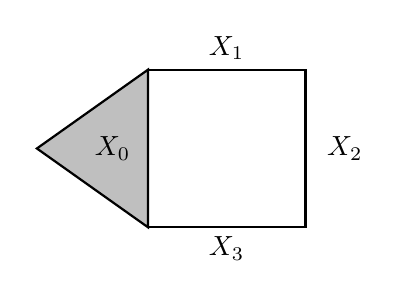
\begin{tikzpicture}
            \draw[thick] (-1, -1) -- (1, -1) -- (1, 1) -- (-1, 1);
            \draw[fill=lightgray, thick] (-1, 1) -- (-1, -1) -- (-2.41, 0) -- cycle;
            \draw (1.5,0) node {$X_{2}$};
            \draw (0,1) node[anchor=south] {$X_{1}$};
            \draw (0,-1) node[anchor=north] {$X_{3}$};
            \draw (-1.1,0) node[anchor=east] {$X_{0}$};
            \draw (-2.41,0) node {\Large $\nodeB$};
            %
            \draw (-1, 1) node {\Large $\nodeW$};
            %
            \draw (1, 1) node {\Large $\nodeR$};
            %
            \draw (1, -1) node {\Large $\nodeW$};
            %
            \draw (-1, -1) node {\Large $\nodeR$};
            %
        \end{tikzpicture}
    \end{minipage}%
    ~\hfil\hfil~ %
    \begin{minipage}{.5\textwidth}
        %
        \begin{tikzcd}
            & w_{1} \arrow[rd, "\text{\Large $\nodeR$}", no head] \arrow["\text{\Large \nodeW, \nodeR}"', no head, loop, distance=2em, in=125, out=55] &          \\
            w_{0} \arrow[ru, "\text{\Large \nodeW}", no head] \arrow[rd, "\text{\Large \nodeR}"', no head] \arrow["\text{\Large \nodeW, \nodeR, \nodeB}"', no head, loop, distance=2em, in=215, out=145] &    & w_{2} \arrow[ld, "\text{\Large \nodeW}", no head] \arrow["\text{\Large \nodeW, \nodeR}"', no head, loop, distance=2em, in=35, out=325] \\
            & w_{3} \arrow["\text{\Large $\nodeW, \nodeR$}"', no head, loop, distance=2em, in=305, out=235]                                     &
        \end{tikzcd}
    \end{minipage} 

        %
        %
        %
        %
        %
        %
    \caption{An impure simplicial model and its corresponding partial epistemic model}
    \label{fig:twoModels}
\end{figure}


\begin{example}
    Figure~\ref{fig:twoModels} depicts a simplicial model $\anglpair{V,S,\coloring,\labSM}$
    (on the left)
    and its corresponding partial epistemic model $\anglpair{M,\sim,L}$ (on the right)
    for $3$ agents with colors $\Ag=\{0,1,2\}$. 
    In the figure, agents $0$, $1$, and $2$ are represented by 
    colored nodes $\nodeW$, $\nodeR$, and $\nodeB$, respectively.  
    Throughout the paper, we will follow this coloring convention.

    For each $i=0,1,2,3$, 
    the facet $X_i$ in the simplicial model corresponds to 
    the possible world~$w_i$ in the partial epistemic model 
    and they have the same set of atomic propositions, i.e., $\ell(X_i) = L(w_i)$. 
    If a pair of facets $X_i$ and $X_j$ share a node of color~$a$, 
    the corresponding possible worlds $w_i$ and $w_j$ are connected by an edge associated 
    with a node of color~$a$, meaning that $w_i \sim_a w_j$.
    Particularly, each possible world $w_i$ has a self-loop colored by $a$ 
    if and only if the agent~$a$ is alive in $w_i$, that is, 
    the corresponding facet $X_i$ contains a vertex colored by~$a$. 
    
    
    %
    %
    %
    %
    %
    %
    %
    %

    %
    %
    %
\end{example}





%

%
%
%
%
%
%
%
%

%

%

%
%

%
%
%
%
%
%
%
%

%
%
%
%
%
%
%
%

%
%

%
%
%
%
%
%
%
%
%
%
%
%
%
%



%
